\documentclass[italian]{beamer}

\usepackage[utf8]{inputenc}
\usepackage[T1]{fontenc}
\usepackage{eurosym}
\usepackage{xcolor}
\usetheme{metropolis}

\usepackage{tikz}
\usepackage{etextools}
\usepackage{adjustbox}
\usetikzlibrary{backgrounds}
\usetikzlibrary{arrows}
\usetikzlibrary{decorations.pathreplacing}

%%%%  MACRO DEFINITION %%%%
\newcommand{\enablebackground}{1} % 0 = disable, 1 = enable
\newcommand{\width}{15}
\newcommand{\height}{12}
\newcommand{\opacity}{0.8}
\newcommand{\mindist}{20}
\definecolor{blueish}{rgb}{0.782,0.943,1}  % blue-ish
\definecolor{lightblueish}{rgb}{0.891,0.971,1}  % lighter blue-ish
\definecolor{darkgreen}{rgb}{0,0.5,0}
\definecolor{lightblue}{rgb}{0.058, 0.784, 0.956}


\tikzset{%
  circlenode/.style={circle, draw=blueish, fill=lightblueish},
  boxnode/.style={rectangle, draw=blueish, fill=lightblueish},
  station/.style={circle, draw=blue, fill=white, minimum size=1cm},
  block/.style={draw=black, fill=lightblue, inner sep=0.4cm, outer sep=0.3cm},
  communicates/.style={implies-implies,double equal sign distance}
}

\tikzstyle{redge}=[draw=blue]


\tikzstyle{transmission}=[decorate, decoration={expanding waves, angle=7,
                          segment length=2}, redge]


\newcommand{\no}{$\mathbin{\tikz [x=1.4ex,y=1.4ex,line width=.2ex, red] \draw (0,0) -- (1,1) (0,1) -- (1,0);}$}%
\newcommand{\ok}{$\color{darkgreen}\checkmark$}

% chktex-file 8

%%%% BACKGROUND CODE %%%%
\makeatletter
\newcommand{\gettikzxy}[3]{ % I got this from https://tex.stackexchange.com/questions/33703/extract-x-y-coordinate-of-an-arbitrary-point-in-tikz
  \tikz@scan@one@point\pgfutil@firstofone#1\relax
  \edef#2{\the\pgf@x}%
  \edef#3{\the\pgf@y}%
}
\newcommand\afteriterationdef[1]{\aftergroup@def#1}
\newcommand\afterforeachdef[1]{\afteriterationdef{#1}\AfterGroup{\aftergroup@def#1}}
\makeatother

\AtBeginSection[]{\frame{\sectionpage}}

% TODO
% https://tex.stackexchange.com/questions/115932/on-the-basics-of-writing-to-reading-from-auxiliary-files-aux-toc-etc
% http://nbeloglazov.com/2015/05/18/trees-quil-and-random.html
\usebackgroundtemplate{%
\ifnum\enablebackground>0
\pgfmathsetseed{\insertframenumber} % DO NOT USE 0 HERE
\adjustbox{min size={\paperwidth}{\paperheight}}{%
    \scalebox{0.6}{
        
\begin{tikzpicture}[inner sep=0.333em, opacity=\opacity]
            \pgfmathparse{random(25, 30)}
            \pgfmathtruncatemacro\nrOfNodes{\pgfmathresult}
            \foreach \i in {1,...,\nrOfNodes} {
                \pgfmathparse{random(0,\width)}
                \pgfmathsetmacro\posX{rnd*\width}
                \pgfmathsetmacro\posY{rnd*\height}
                \ifnum\mindist>0
                    \ifnum\i>1
                        \pgfmathtruncatemacro\imo{\i-1}
                        \node (a-\i) at (\posX, \posY) {};
                        \gettikzxy{(a-\i)}{\pX}{\pY};
                        \foreach \cnt in {1,...,20} {
                            \pgfmathtruncatemacro\isok{1}
                            \foreach \j in {1,...,\imo} {
                                \gettikzxy{(a\j)}{\qX}{\qY};
                                \pgfmathsetmacro\diffX{(\pX-\qX)/100}
                                \pgfmathsetmacro\diffY{(\pY-\qY)/100}
                                \pgfmathtruncatemacro\calculatedDistance{100*sqrt((\diffX)^2 + (\diffY)^2)};
                                \ifnum\calculatedDistance<\mindist
                                    \pgfmathtruncatemacro\isok{0}
                                    \afterforeachdef\isok
                                    \breakforeach
                                \fi
                            }
                            \ifnum\isok=1
                                \breakforeach
                            \else
                                \pgfmathsetmacro\posX{rnd*(\width)}
                                \pgfmathsetmacro\posY{rnd*(\height)}
                                \afterforeachdef\posX
                                \afterforeachdef\posY
                            \fi
                        }
                    \fi
                \fi
                \pgfmathparse{random(0, 3)}
                \pgfmathtruncatemacro\nodetype{\pgfmathresult}
                \ifnum\nodetype>0
                    \node [circlenode] (a\i) at (\posX, \posY) {};
                \else
                    \node [boxnode] (a\i) at (\posX, \posY) {};
                \fi
            }
            \begin{pgfonlayer}{background}
                \begin{scope}[opacity=\opacity]
                    \foreach \i in {1,...,\nrOfNodes} {
                        \pgfmathsetmacro\ipo{\i+1}
                        \ifnum\i<\nrOfNodes
                            \foreach \j in {\ipo,...,\nrOfNodes} {
                                \gettikzxy{(a\i)}{\pX}{\pY};
                                \gettikzxy{(a\j)}{\qX}{\qY};
                                \pgfmathsetmacro\diffX{(\pX-\qX)/100}
                                \pgfmathsetmacro\diffY{(\pY-\qY)/100}
                                \pgfmathtruncatemacro\calculatedDistance{4+max(20*((\diffX)^2 + (\diffY)^2) - 15, 0)};
                                \pgfmathparse{random(0, \calculatedDistance)}
                                \pgfmathtruncatemacro\hasarc{\pgfmathresult}
                                %\pgfmathparse{random(0, 20)}
                                %\pgfmathsetmacro\curveangle{atan2(\qY-\pY, \qX-\pX)-\pgfmathresult+10}
                                \ifnum\hasarc<3
                                    %\draw[blueish] (a\i) to[in=-\curveangle,out=\curveangle] (a\j);
                                    \draw[blueish] (a\i) to (a\j);
                                \fi
                            }
                        \fi
                    }
                \end{scope}
            \end{pgfonlayer}
        \end{tikzpicture}
    }
}
\fi
}%


\author{Luca Versari}
\title{Smart light management in a house}
\begin{document}
\frame{\titlepage}

\section{Project objective and requirements}
\begin{frame}{Project objective}
    Automatize lights' on/off status
    \begin{itemize}
        \item<2-> Computer-based (or app-based) management (\ok)
        \item<3-> Automatically turn a light on for a while when a person walks in a room (\ok)
        \item<4-> \dots if it's dark outside (\ok)
    \end{itemize}
\end{frame}

\begin{frame}{Requirements}
    \begin{itemize}
%        \item<1-> Devices that aren't hidden in a wall should have no visible wires
        \item<1-> Battery-backed devices should last for (at least) months
        \item<2-> The system should be very fault tolerant (\ok)
        \item<3-> It should be possible to ``rewire'' the switches easily (\ok)
    \end{itemize}
\end{frame}

\section{Hardware setup}
\begin{frame}{Hardware overview}
    There are three devices in use (so far!)
    \begin{itemize}
        \item<1-> A \textit{node} is a device that has sensors and/or actuators attached
        \item<2-> The \textit{sink} is the (unique) device that gathers information from nodes (and sends external commands)
        \item<3-> The \textit{gateway} is the node that exposes a web interface to manage the system
        \item<4-> (planned) A \textit{battery node} is the same as a node, except that it only has sensors and it is battery-backed.
    \end{itemize}
\end{frame}

\begin{frame}{Components used}
    \begin{itemize}
        \item<1-> The nodes (and the sink) use an \textit{Atmega328p}, aka. Arduino.
        \item<2-> Wireless communication is handled via the \textit{nrf24l01+} module.
        \item<3-> The gateway will be a (Raspberry|Orange|Banana) Pi.
        \item<4-> Communication between the sink and the gateway happens via serial port.
    \end{itemize}
\end{frame}

\section{Software setup}
\begin{frame}{Software setup}
    \centering
    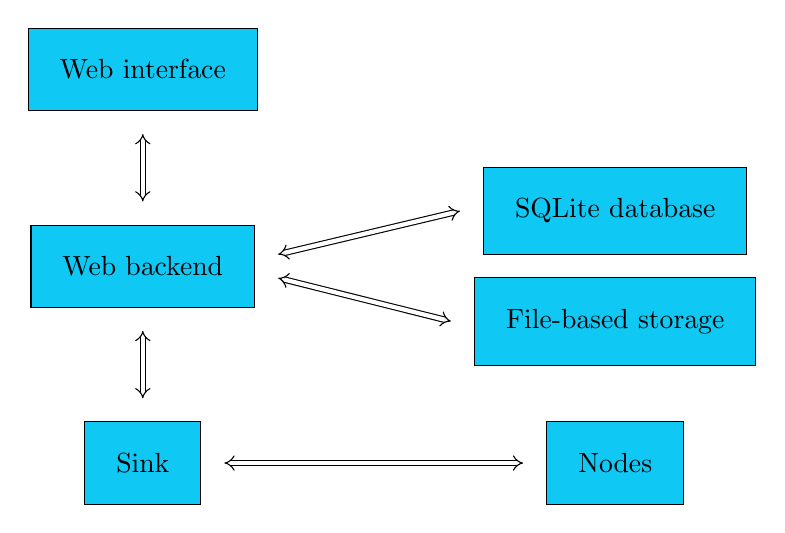
\begin{tikzpicture}[node distance=2.5cm]
        \node [block]                                                  (wui) {Web interface};
        \node [block, below of=wui]                                    (wbk) {Web backend};
        \node [block, right of=wbk, node distance=6cm, yshift=0.7cm]   (sql) {SQLite database};
        \node [block, right of=wbk, node distance=6cm, yshift=-0.7cm]  (fbs) {File-based storage};
        \node [block, below of=wbk]                                    (snk) {Sink};
        \node [block, below of=sql, yshift=-0.7cm]                     (nds) {Nodes};

        \draw [communicates] (wui) -- (wbk);
        \draw [communicates] (sql.west) -- (wbk.5);
        \draw [communicates] (fbs.west) -- (wbk.355);
        \draw [communicates] (snk) -- (wbk);
        \draw [communicates] (snk) -- (nds);
    \end{tikzpicture}
\end{frame}

\begin{frame}{Web backend}
    \begin{itemize}
        \item <1-> Written in Javascript using JQuery
        \item <2-> Communicates using AJAX
        \item <3-> Allows to turn on/off single switches, and to configure devices that join the network
            \begin{itemize}
                \item<4-> Set which buttons/PIRs turn on a specific switch
                \item<5-> Set how long the detection of motion through a PIR should leave the switch on
            \end{itemize}
    \end{itemize}
\end{frame}

\begin{frame}{Web interface}
    \begin{itemize}
        \item <1-> Written in Rust
        \item <2-> Stores the network configuration on a file
        \item <3-> Stores events on a SQLite database
            \begin{itemize}
                \item<4-> Button press
                \item<5-> PIR activation
                \item<6-> Light status
            \end{itemize}
        \item <7-> Uses the serial port to communicate with the sink
    \end{itemize}
\end{frame}

\begin{frame}{Sink}
    \begin{itemize}
        \item <1-> Translates messages received on the wireless to the serial port and vice-versa.
        \item <2-> The format of messages on the serial port is kept as simple as possible:
            \begin{itemize}
                \item <3-> Fixed width
                \item <4-> A magic byte ($123$) that signals the start of a message
                \item <5-> A byte representing the kind of message
                \item <6-> Message data ($4$ or $5$ bytes depending on the direction)
            \end{itemize}
    \end{itemize}
\end{frame}

\begin{frame}{Node}
    \begin{itemize}
        \item <1-> Up to $2$ switches
        \item <2-> Up to $5$ buttons
        \item <3-> Up to $2$ PIRs
        \item <4-> An (optional) \textit{PIR controller}: a sensor that may inhibit the activation
            of the connected PIRs (for example, when there is a lot of ambient light)
        \item <5-> Each node has a unique ID set at compile-time.
        \item <6-> The system is fully modular: the software may handle any valid configuration
            with the same compile-time configuration
        \item <7-> Switch configuration is saved on the EEPROM to persist across power outages
        \item <8-> The switch broadcasts events as they happen and broadcasts its status every
            now and then
    \end{itemize}
\end{frame}

\section{Wireless communication}
\begin{frame}{Overview}
    Wireless communication uses two layers:
    \begin{itemize}
        \item<1-> Broadcast layer, that sends a message to everybody else in the network
        \item<2-> Application layer, that uses the broadcast layer to communicate
    \end{itemize}
    \uncover<3>{The application layer uses fixed-size messages and is fairly straightforward.
    The main challenge is the \textit{broadcast layer}.}
\end{frame}

\begin{frame}{Multi-hop}
    Nodes may not all be within range of each other:
    \vspace{1cm}
    \begin{center}
        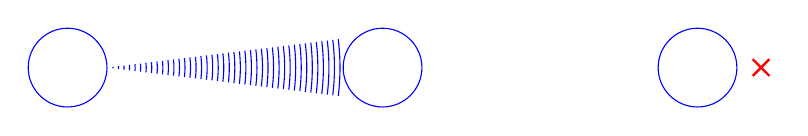
\begin{tikzpicture}[node distance=4cm]
            \node [station]                  (source) {};
            \node [station, right of=source] (dest1) {};
            \node [station, right of=dest1]  (dest2) {};

            \uncover<4>{\node at ([xshift=0.3cm]dest2.east) {\no};}

            \draw<2> [transmission] (source) -- (dest1);
        \end{tikzpicture}
    \end{center}
\end{frame}

\begin{frame}{Collisions}
    The trivial attempt does not work so well:
    \vspace{1cm}
    \begin{center}
        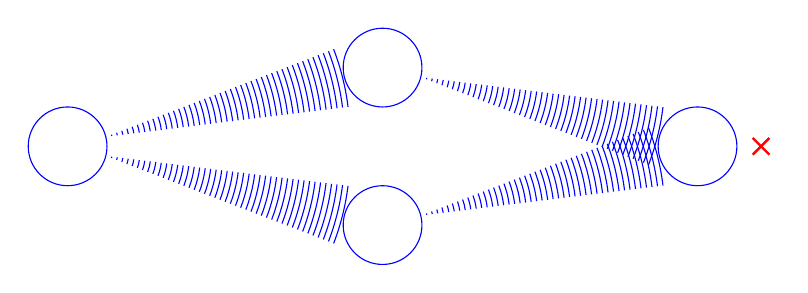
\begin{tikzpicture}[node distance=4cm]
            \node [station]                               (source) {};
            \node [station, right of=source,yshift=1cm]   (dest1) {};
            \node [station, right of=source,yshift=-1cm]  (dest2) {};
            \node [station, right of=dest1,yshift=-1cm]  (destU) {};

            \uncover<5>{\node at ([xshift=0.3cm]destU.east) {\no};}

            \draw<2> [transmission] (source) -- (dest1);
            \draw<2> [transmission] (source) -- (dest2);
            \draw<4-5> [transmission] (dest1) -- (destU);
            \draw<4-5> [transmission] (dest2) -- (destU);
        \end{tikzpicture}
    \end{center}
\end{frame}

\begin{frame}{Solution}
    \begin{itemize}
        \item<1-> Each node transmits every new packet a constant number ($16$) of times
        \item<2-> Between two transmissions, they wait a random amount of time (using
            a rng seeded with the ID of the node)
        \item<3-> Received packets are de-duplicated by checking them against the last
            ones received.
        \item<4-> When transmitting, we periodically empty the receive buffer of the
            network card to avoid losing packets to full buffers.
        \item<5-> An autoincrementing number is prepended to the outgoing packet
            to allow to send packets with the same content.
    \end{itemize}
\end{frame}

\section{Demo}
\begin{frame}{Demo}
    \begin{itemize}
        \item<1-> Two nodes, one sink and one gateway
        \item<2-> One node has five buttons and two switches (that control a red and a green LED)
        \item<3-> The other has a button, a PIR, a light sensor and a switch (that controls a yellow LED)
        \item<4-> We'll try the sensors and the web interface
        \item<5-> If the room allows, we'll try multi-hop communication
        \item<6-> You can find the code on GitHub: \url{https://github.com/veluca93/light_manager}
    \end{itemize}
\end{frame}
\end{document}
